\pagestyle{fancy}
\headheight 20pt
\lhead{Ph.D. Thesis --- R. Woods}
\rhead{McMaster - Physics \& Astronomy}
\chead{}
\lfoot{}
\cfoot{\thepage}
\rfoot{}
\renewcommand{\headrulewidth}{0.1pt}
\renewcommand{\footrulewidth}{0.1pt}

\chapter{The Numerical Method}
\label{chap:method}
\thispagestyle{fancy}

In the absence of absorbing material, the problem of radiative transfer reduces down to that of gravity. As such, the tree-algorithm for calculating gravity can be used \citep{barnesHut86}.

\begin{itemize}
\item A tree can be used to partition space.
\item Each level of the tree holds finer partitions of the volume. See figure \ref{fig:trees}
\item Each node of the tree contains accumulated information about the tree below it (total mass, etc.).
\item In order to calculate gravity on a particular leaf (bucket), you can interact with the moment of another cell (\ref{eq:gravitymoments}).
\item To decide what level of the tree to interact with, you can define an opening angle/radius, $\theta$. If a cell is smaller than this opening angle (the distribution of matter inside the cell is contained within a small enough angle on the sky), the entire cell can be used in the force calculation. If not, you must consider the child nodes separately. See equation \ref{eq:openingangle}.
\item On average, the number of interactions a each particle will have is $\log{N}$, where N is the total number of particles. Thus, the force calculation for the whole simulation scales as $N\log{N}$. Note that lowering $\theta$ shifts the number of calculations that are approximated by large cells to smaller cells, and thus if $\theta$ is very small, the code approached scaling of order $N^2$.
\item In the case of radiation, the math is very similar (See eq \ref{eq:radiationmoments}). However, since radiation does not cancel like forces, the dipole moment does not disappear and a rougher approximation is possible (wording wrong, fix this).
\item In this case, the interaction scales as $N_{\mbox{sink}}\log{N_{\mbox{source}}}$. However, assuming the full tree is still used, the tree-build still scales as $N\log{N}$.
\end{itemize}

\begin{equation}
\label{eq:gravitymoments}
\Phi = \frac{G}{4\pi}\sum\limits_{n=0}^{\infty} \frac{1}{r^{(n+1)}}\int (r')^n P_n (\cos{\theta '}) \rho(\boldsymbol r') d\tau '
\end{equation}

\begin{equation}
\label{eq:radiationmoments}
F = \frac{L}{4 \pi r^2}
\end{equation}

\section{Tree Data Structures}
\label{sec:treestruct}

In order to understand the radiative transfer algorithm that we are presenting, it is important to understand tree data structures.

\begin{itemize}
\item Terminology: Node, root node, leaf node, interior node, child, parent, sibling, tree build, walk the tree, ascend the tree, descend the tree.
\item In computer science, a tree is a hierarchical data structure. Typically the tree starts at a single point, usually called the root node, and branches out to many other ``child'' nodes.
\item Each node in the tree stores some sort of data, and the relative location of the node in the tree indicates the relation of the data in the node to the data in other nodes.
\item \textsc{Gasoline} uses a ``k-d tree'' for gravity. This is an example of a binary space-partitioning tree. Every node contains 2 children, and each node of the tree represents a particular volume of space. kd-Trees and octrees represent the majority of trees used in astrophysical simulations. See figure \ref{fig:trees} for visual examples of trees.
\end{itemize}

\begin{figure}
        \centering
        \begin{subfigure}[b]{0.45\textwidth}
                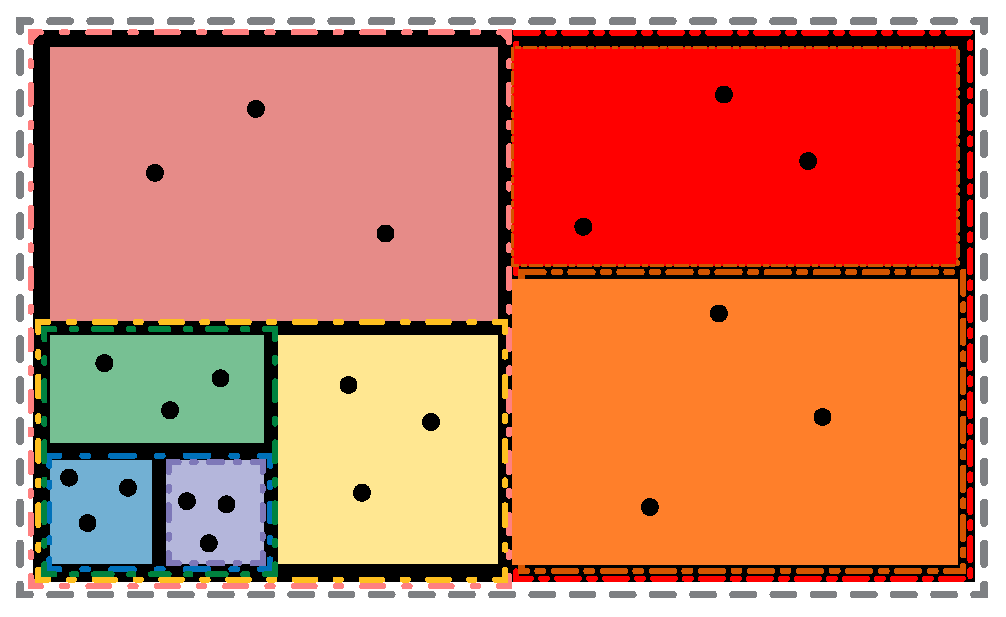
\includegraphics[width=\textwidth]{graphics/tree.eps}
                %\caption{A representation of the algorithm in real space, with the tree overlaid.}
                \label{fig:volumetree}
        \end{subfigure}
        ~ 
        \begin{subfigure}[b]{0.45\textwidth}
                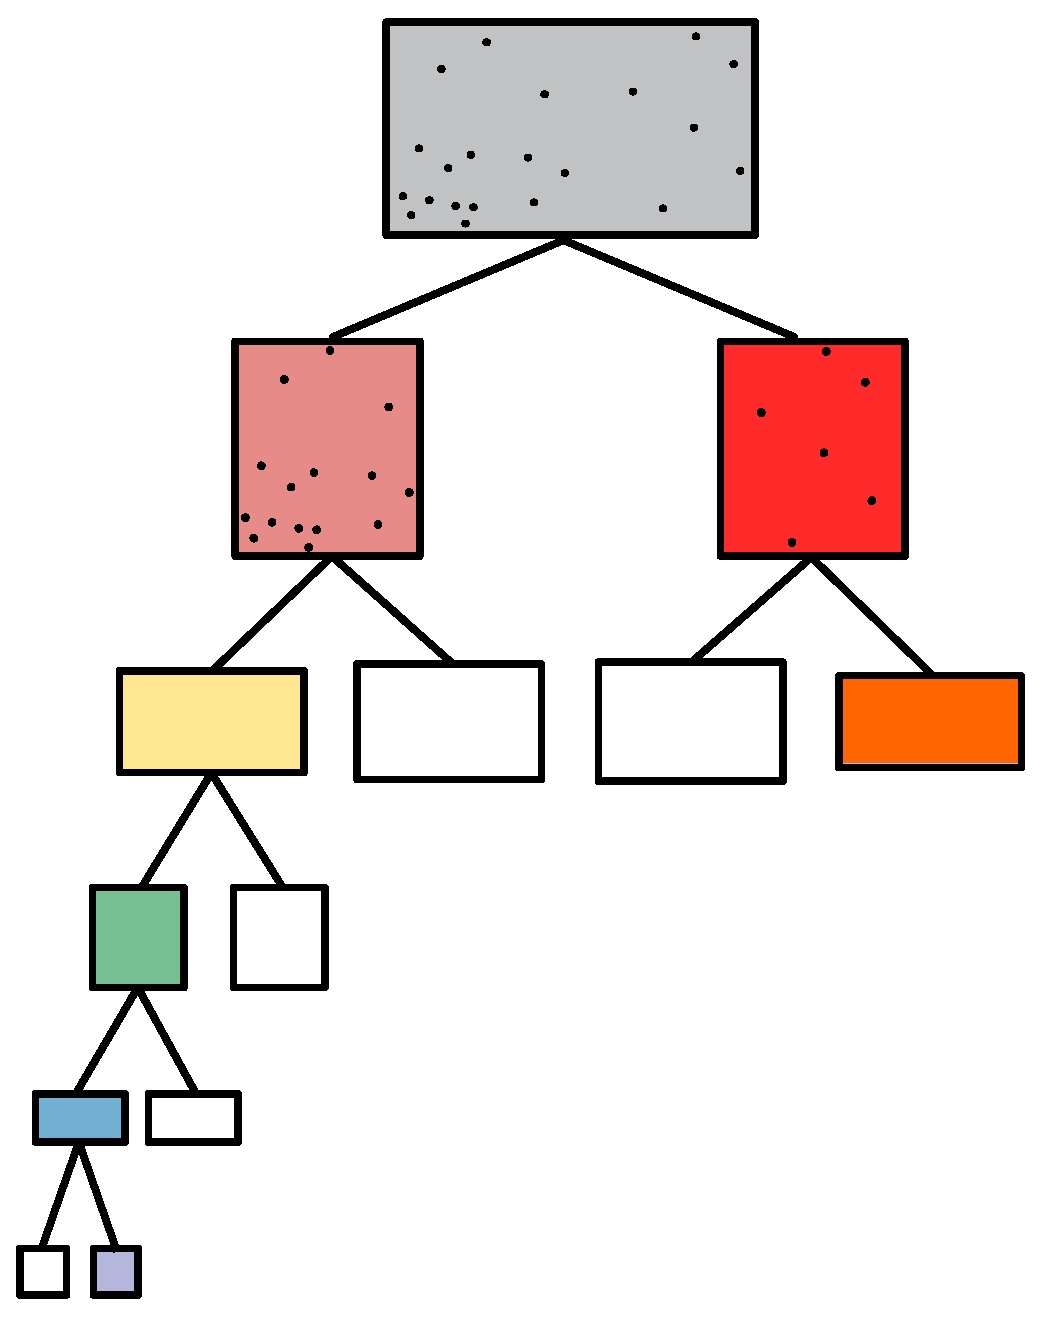
\includegraphics[width=\textwidth]{graphics/tree_memory.eps}
                %\caption{The colors correspond to the volumes on the left.}
                \label{fig:memorytree}
        \end{subfigure}
        \caption[Example of trees]{This is an example of a binary tree. The volume is represented by a tree node, and each volume is then split into two subvolumes, which are represented by two ``child'' nodes of the original node. This splitting can continue indefinitely on either side, making the tree an effective way at splitting volumes.}\label{fig:trees}
\end{figure}

\section{Building a Radiation Tree}
\label{sec:buildingtree}

\begin{itemize}
\item While the algorithm we present is general enough to work with any volume-filling tree, the following sections will introduce the algorithm as we have developed it. \textsc{Gasoline} uses a k-d tree for its gravity solver, and as such, our version of the algorithm uses this tree type in order to make use of existing tools in the code base.
\item The recursive pseudocode for the tree-build is presented below (note - change to nice pseudocode format):
	\begin{enumerate}
	\item if number of data elements greater than n$_{\mbox{leaf}}$, partition data
	\item recursively call build tree on each partition of the data set
	\item else, if number of data elements less than n$_{\mbox{leaf}}$, calculate basic cell properties
	\item After if statement, calculate accumulated cell properties (higher moments, etc)
	\end{enumerate}
\item In our case, the partition data step involves finding the longest axis of the data contained on the current node and dividing particles to the upper and lower halves of the midway point of that axis.
\item Each volume and its corresponding list of particles is then passed recursively to the tree build function again. This terminates when build tree receives a list of particles that is sufficiently short (less than a user set parameter, n$_{\mbox{leaf}}$). At this point, basic cell properties such as center of luminosity and total luminosity are calculated.
\item Once the leaf nodes have been calculated, more complicated average properties, such as higher moments, can be calculated by looping through all particles in the node. This applies to both leaf and interior nodes.
\item The initial partition function does not require that the data be fully sorted, only that it be divided to either side of an intermediate value. This is an order n operation.
\item The tree will be roughly of depth $\log(N)$, meaning that the partition will need to be performed $\log{N}$ times. Therefore, the tree build should scale as roughly $N\log{N}$.
\item For radiation, average cell properties that are used are average density, average opacity, standard deviation of opacity, total luminosity, and center of luminosity.
\item Note that we have calculated center of luminosity without taking into account absorption within the cell.
\end{itemize}

\section{Exchanging Radiation}
\label{sec:exchangerad}
Once the tree has been built, calculating the radiation (gravity) at any particular point can be accomplished by traversing the tree structure, a process called a ``tree walk.''

\begin{itemize}
\item First, a ``post-order'' tree walk is performed in which the children of a node are always checked before its sibling. The walk continues until it arrives at a leaf node, at which point the radiation (gravity) arriving at that leaf is calculated. This leaf node will be called the receiving leaf.
\item The second walk occurs during the radiation (gravity) calculation. We must check what cells are acceptable to interact with based on the opening angle criteria mentioned in the chapter \ref{chap:method} introduction. We can make use of the fact that no children below a cell that has already accepted the $\theta$ criterion need be checked, as they are contained within the cell and so automatically satisfy the criteria of their parent.
\item The algorithm looks like:
	\begin{enumerate}
	\item Given a cell (starting with the root cell), check if the distance, r, from the current leaf to the cell is shorter than the opening radius (given by equation \ref{eq:openingradius}).
	\item If r is shorter than the opening radius, the cell must be ``opened,'' meaning that we return to step 1, but now passing in each child node to check.
	\item If r is longer than the opening radius, the cell is acceptable to interact with. The radiation may be calculated to the bucket using equation \ref{eq:bucketflux}. See figure \ref{fig:openinganglecriteria}.
	\item In the case that the distance to the cell is smaller than the opening radius, and the node has no children (e.g. for leaves of the tree that are very spatially close to the receiving leaf), the interaction should not be approximated, and the direct n$^2$ summation over all particles in each leaf is performed.
	\item Once radiation has been calculated from the current cell, the tree-walk is allowed to skip all children of the current cell and move on to its sibling or parent's sibling (parent's sibling in the case that we are the right-hand child of the parent node). 
	\end{enumerate}
\item Once radiation has been calculated for the receiving bucket, we move on to the next bucket, which is accomplished by moving to the sibling if the current bucket is the left child of the parent node, or to the sibling of the parent node if we are the right child. An example radiation exchange is shown in figure \ref{fig:radexchange}.
\item The above algorithm will run in $N\log{N}$ time, as with gravity. However, unlike gravity, not all objects emit radiation. Thus, technically the more specific scaling is $N_{\mbox{sink}}\log{N_{\mbox{source}}}$. The slow growth rate of computation time with the number of sources makes the algorithm a very strong candidate for cosmological applications in which there are often similar numbers of star particles to gas particles. In fact, some codes have already made use of this basic idea \citep{gnedinAbel01,hopkins, kannanEt14}. As well, the algorithm may allow for the treatment of gas particles as sources (more caerful considerations must be made to tie the radiation to the cooling of the gas in this case), which is rarely done due to incredibly high computational cost.
\end{itemize}

\begin{equation}
\label{eq:openingangle}
\theta_{\mbox{crit}} = \frac{b_{\mbox{max}}}{r}
\end{equation}

\begin{equation}
\label{eq:openingradius}
r_{\mbox{crit}} = \frac{b_{\mbox{max}}}{\theta_{\mbox{crit}}}
\end{equation}

\begin{equation}
\label{eq:bucketflux}
F_{\mbox{bucket}} = \frac{L_{\mbox{tot}}}{4\pi r^2}e^{-\tau}
\end{equation}

\begin{figure}
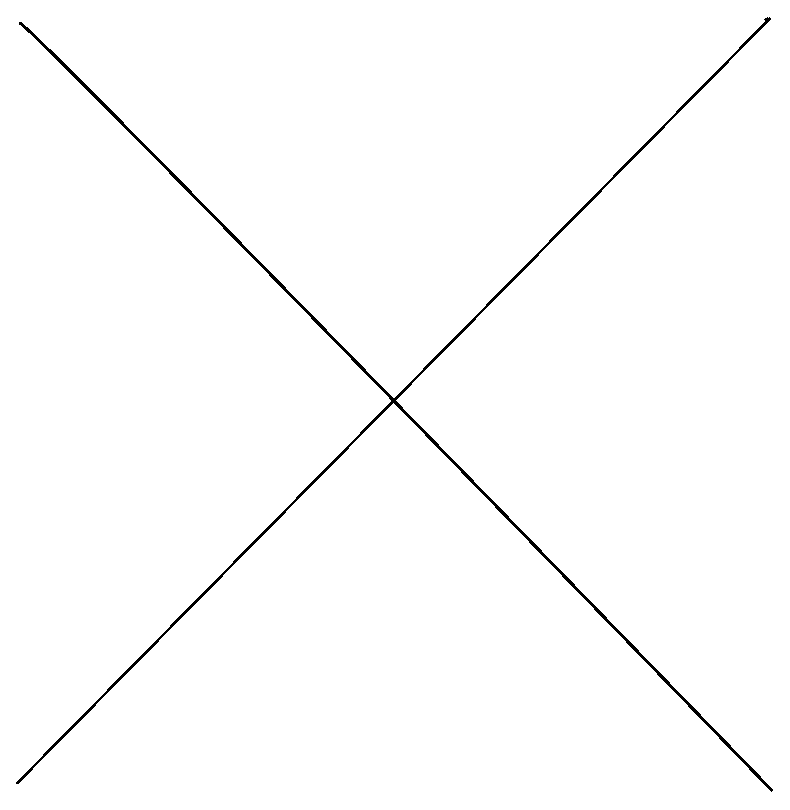
\includegraphics[width=\textwidth]{graphics/placeholder.eps}
\caption[The opening angle criteria.]{Cell A in this image is the receiving cell, while cells B, C, and D are cells that A will receive flux from. Cell A is close enough so that it should be opened, but is a leaf and so it requires a direct $n^2$ summation. Cell C is close enough and is not a leaf, so it will have its two children checked for the same criteria (the left child will be too close, the right child will be acceptable to interact with). Cell D is not a leaf, but is sufficiently far away that leaf A can interact with the full cell.}
\label{fig:openinganglecriteria}
\end{figure}

\begin{figure}
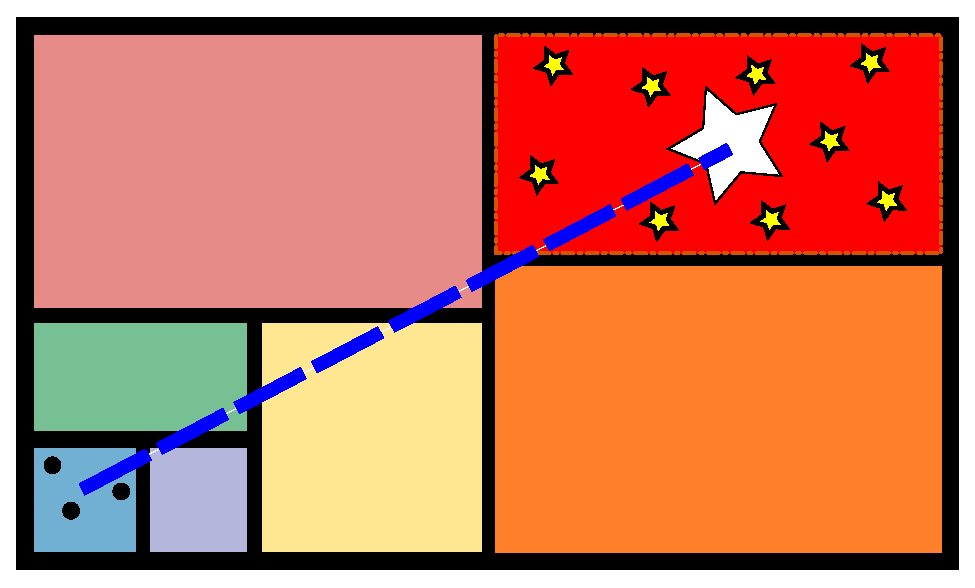
\includegraphics[width=\textwidth]{graphics/flux.eps}
\caption[The exchange of radiation.]{In this image, cell A is receiving radiation from cell B. Cell B is sufficiently far away that we can find the center of luminosities of all the sources inside of it, and calculate flux based on that single value rather than summing each one individually.}
\label{fig:radexchange}
\end{figure}

\section{Absorption}
\label{sec:absorption}

The algorithm presented in sections \ref{sec:buildingtree} and \ref{sec:exchangerad} assumes that no change to the radiation (force) happens in between the sending and receiving buckets. In gravity, this is acceptable because forces are not ``absorbed'' in any way. However, radiation tends to be absorbed and scattered by intervening material and thus the intensity of the radiation at a point is not only due to the sending source, but to all material in between the source and the sink.

\begin{itemize}
\item As mentioned in chapter \ref{chap:intro}, most current radiative transfer codes either completely ignore intervening material or do very detailed tracing of photons throughout the medium. The former option produces very bad radiation fields while the latter is incredibly computationally expensive.
\item In order to reproduce the behavior of equation \ref{eq:radtransfer}, we must modify the algorithm to be able to find the optical depth between any two points. However, we must be careful not to lose the performance afforded by the tree. In order to do this, we have developed the algorithm to make use of the tree during the optical depth calculation as well.
\item The crucial point to the algorithm lies in the fact that for any two interacting cells, there exists a common parent node. Thus, all intervening space between the cells must lie within the subtree in which the common parent is the root.
\item If we traverse up the depth of the tree (hereafter referred to as a tree climb) once from each interacting node to the common parent node, we will have performed roughly $\log(N)$ extra operations per interaction. If we do no other work than this, then our scaling for radiative transfer changes to $N_{\mbox{sink}}\log{N_{\mbox{source}}}\log{N}$. While the extra factor of $\log{N}$ is certainly worth noting, it does not tend to increase scaling by a significant amount.
\item Our goal then becomes to perform order (1) amount of work during this additional tree climb.
\item In order to accomplish this, we need only make use of the average properties recorded for each cell during the tree build.
\item At each higher cell during the tree climb, we obtain a larger representative volume from that cell. The new volume contains the previous volume as well as a new contribution from the previous cell's sibling. This sibling's volume may or may not lie on the vector connecting the two interacting cells. This can be determined by calculating the distance to the edge of the current volume along the vector from the centers of the original interacting cells. This operation is completed in order (1) time. (introduce this algorithm?).
\item At each new higher cell, if the calculated line segment is longer than the accumulated distance so far, than the difference is the amount of the vector contained in the additional volume. By recording this new line segment, the average density of the cell, and the average opacity of the cell (both values that were accumulated during the tree build), then we have everything needed to calculate the optical depth of the line segment according to equation \ref{eq:opticaldepth}. By summing the optical depth of each line segment, we will have obtained the full optical depth between the interacting cells in order $log{N}$ time. The algorithm is depicted graphically in figure \ref{fig:absorption}
\end{itemize}

%\begin{figure}
%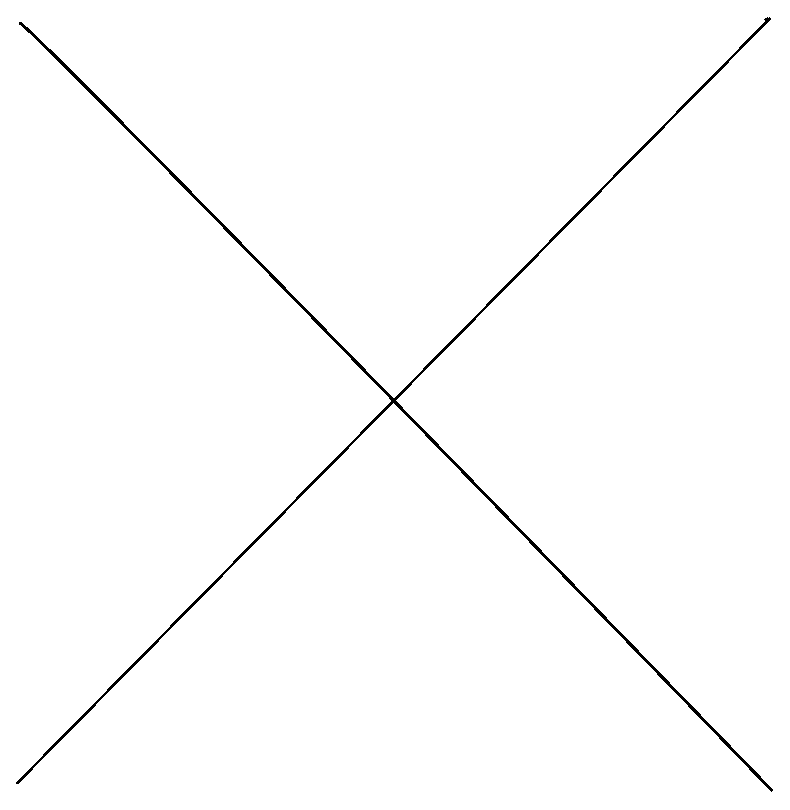
\includegraphics[width=\textwidth]{graphics/placeholder.eps}
%\caption{}
%\label{fig:absorption}
%\end{figure}

\begin{figure}
        \centering
        \begin{subfigure}[b]{0.45\textwidth}
                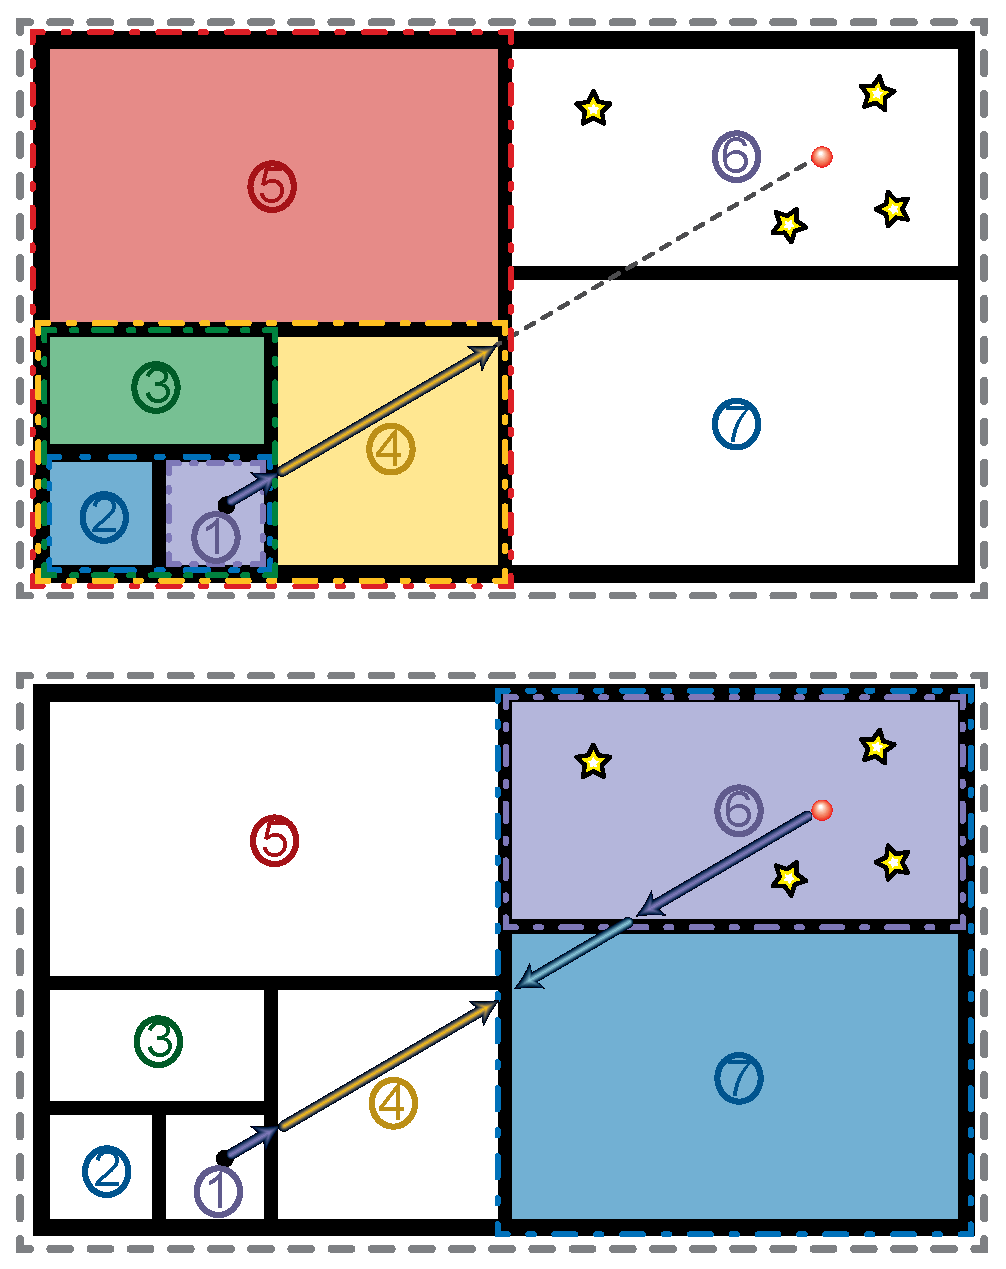
\includegraphics[width=\textwidth]{graphics/RT_algorithm.eps}
                \caption{A representation of the algorithm in real space, with the tree overlaid.}
                \label{fig:treeclimb}
        \end{subfigure}
        ~ 
        \begin{subfigure}[b]{0.45\textwidth}
                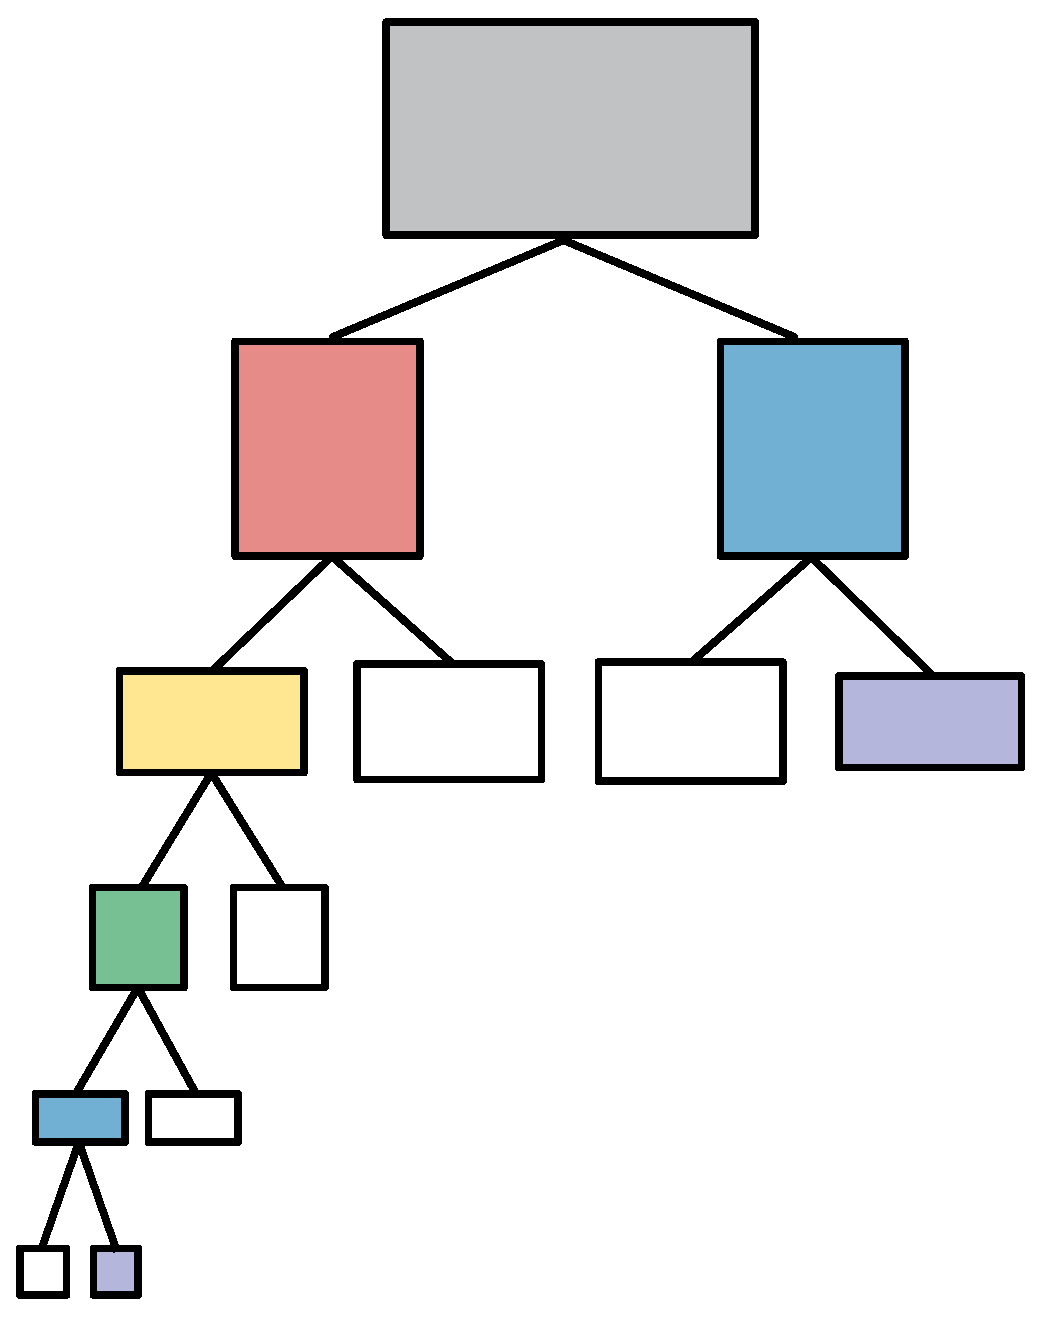
\includegraphics[width=\textwidth]{graphics/RT_tree.eps}
                \caption{The colors correspond to the volumes on the left.}
                \label{fig:absorptiontree}
        \end{subfigure}
        \caption[The absorption algorithm.]{The absorption algorithm.}\label{fig:absorption}
\end{figure}

\section{Refinement}
\label{sec:refinement}

While section \ref{sec:absorption} introduces a very fast algorithm for calculating a radiation field, it relies heavily on the geometry of the underlying tree. In volumes with very smooth density/opacity, the above algorithm performs very well. However, in cases with sharp density/opacity gradients, the density/opacity gradient is discretized into widths of order the cell size at the current tree depth. This can become problematic, causing the tree structure to be imposed into the calculated radiation field. In order to solve this, we introduce a refinement process to the algorithm that allows a descent back down the tree during the tree climb in order to obtain a more detailed description of the medium.

\begin{itemize}
\item The refinement is a fairly straightforward addition to the algorithm. At the point where the average properties of the cell would normally be considered, we simply check if the current cell passes a refinement criteria.
\item If the cell passes the criteria to refine, rather than recording the average properties, we recursively check the children of section of the tree we did \emph{not} ascend from.
\item Once we arrive at a cell that fails the criteria to refine (or at a leaf and can no longer refine), we record the line segment within the cell and the average properties as normal, and return up the recursive call. See figure \ref{fig:refining} for a visual representation.
\item The specific refinement criteria has deliberately been left vague until this point. In principle, one can refine on any cell property desired.
\item For the purposes of this paper, we have decided to use an opacity refinement criteria. Within any cell, if a constant times the standard deviation of the average opacity is larger than the average opacity, the cell is refined. We find this produces a reasonable amount of refinement in code tests.
\item Note that this is not necessarily the ideal criteria for physical simulations. It would be wise not only to look at the variation in opacity, but also the absolute value. In cases where the optical depth is very high, most of the radiation will be absorbed anyway, and the algorithm can be terminated since this particular vector yields a negligible flux of photons to the receiving cell.
\end{itemize}

\begin{figure}
        \centering
        \begin{subfigure}[b]{0.45\textwidth}
                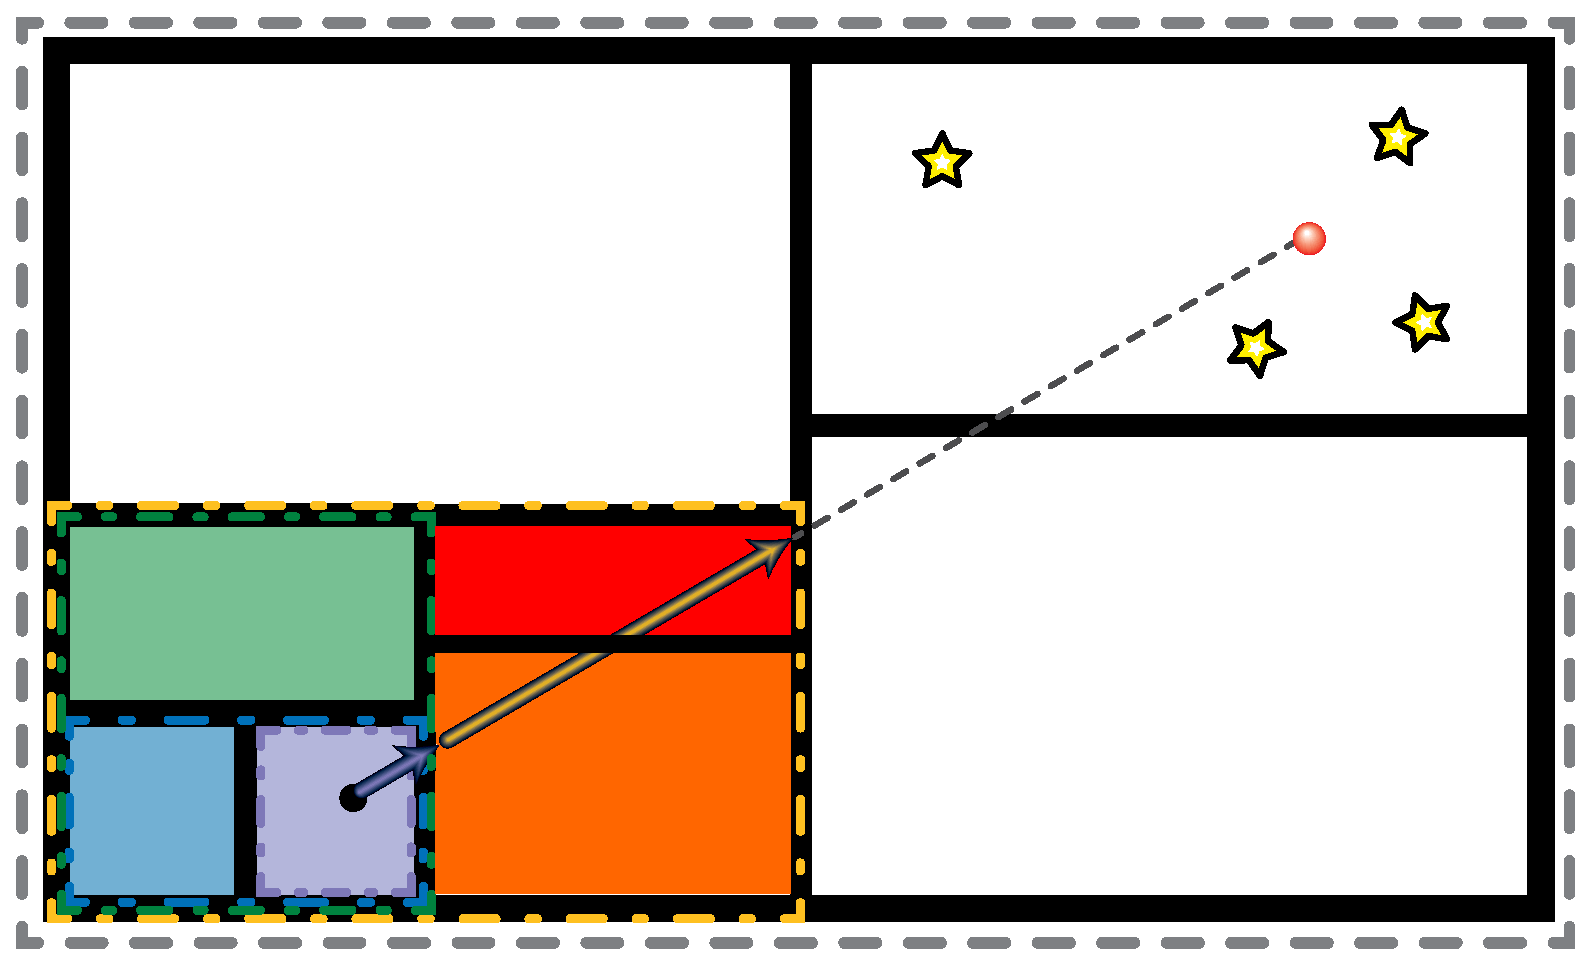
\includegraphics[width=\textwidth]{graphics/refinement.eps}
                \caption{The tree splits the line segment into the red and orange sections.}
                \label{fig:refinetree}
        \end{subfigure}
        ~ 
        \begin{subfigure}[b]{0.45\textwidth}
                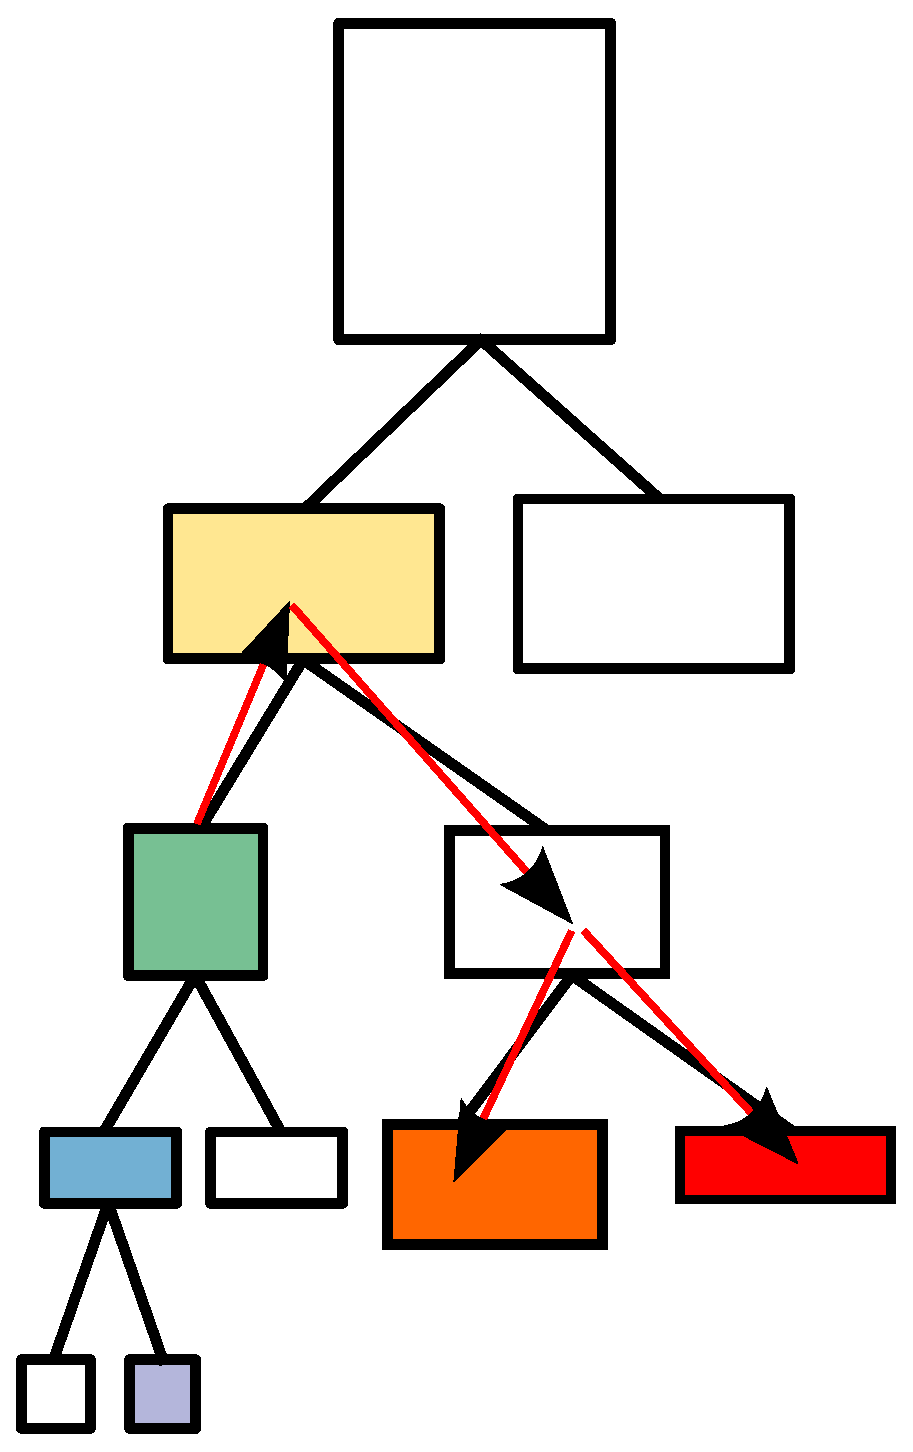
\includegraphics[width=\textwidth]{graphics/refine_memory.eps}
                \caption{The colors correspond to the volumes on the left.}
                \label{fig:refinememory}
        \end{subfigure}
        \caption[Refinement during the absorption algorithm.]{When the line segment is too rough in some physical sense, refinement can be triggered. Visually, the algorithm descends back down the tree the opposite direction it came from until the criteria to refine is no longer satisfied or until a leaf is reached.}\label{fig:refining}
\end{figure}



Extension of the refinement to ray-tracing
\begin{itemize}
\item If very high accuracy is required, the refinement routine is flexible enough that sub-leaf refinement is possible. While this has not currently been tested since it leaves the regime of low computational expense, it could easily be implemented.
\item If a leaf was reached during refinement and still passed the criteria to be refined on, the individual particles inside the cell could be considered.
\item A ray tracing scheme through the cell similar to SPHRay \citep{altayEt08} could be performed. The machinery to do this ray trace is already established for use within the receiving and sending cells (see section \ref{sec:resolvingleaves} and figure \ref{fig:raytracing}).
\end{itemize}

\section{Resolving the Receiving Cells}
\label{sec:resolvingleaves}

During testing, we ran into issues with ionization fronts ``stalling'' in certain cells. If a sharp ionization front is passing through a receiving bucket, then the effects of averaging can cause issues if the optical depth of the bucket is of order unity or higher. (below section needs re-wording and more specifics).

\begin{itemize}
\item Consider an ionization front that has passed halfway through a leaf node (half of the particles are ionizaed, half are not).
\item The average opacity will be $\kappa/2$, where $\kappa$ is the opacity of the unionized particles.
\item The ionized particles will use an opacity that is much too large, therefore reducing the flux that particles at the ``rear'' of the leaf see.
\item This means that particles at the rear of the leaf are harder to ionize than at the front, and the propagation speed of the front is drastically reduced.
\item In order to combat this, more detailed tracing is required \emph{only in the receiving leaf}.
\item This is easily accomplished by implementing a scheme similar to SPHRay \citep{altayEt08}. (introduce simpler method that we use where we order particles along vector and linearly add optical depth?). See figure \ref{fig:raytracing}.
\end{itemize}

\begin{figure}
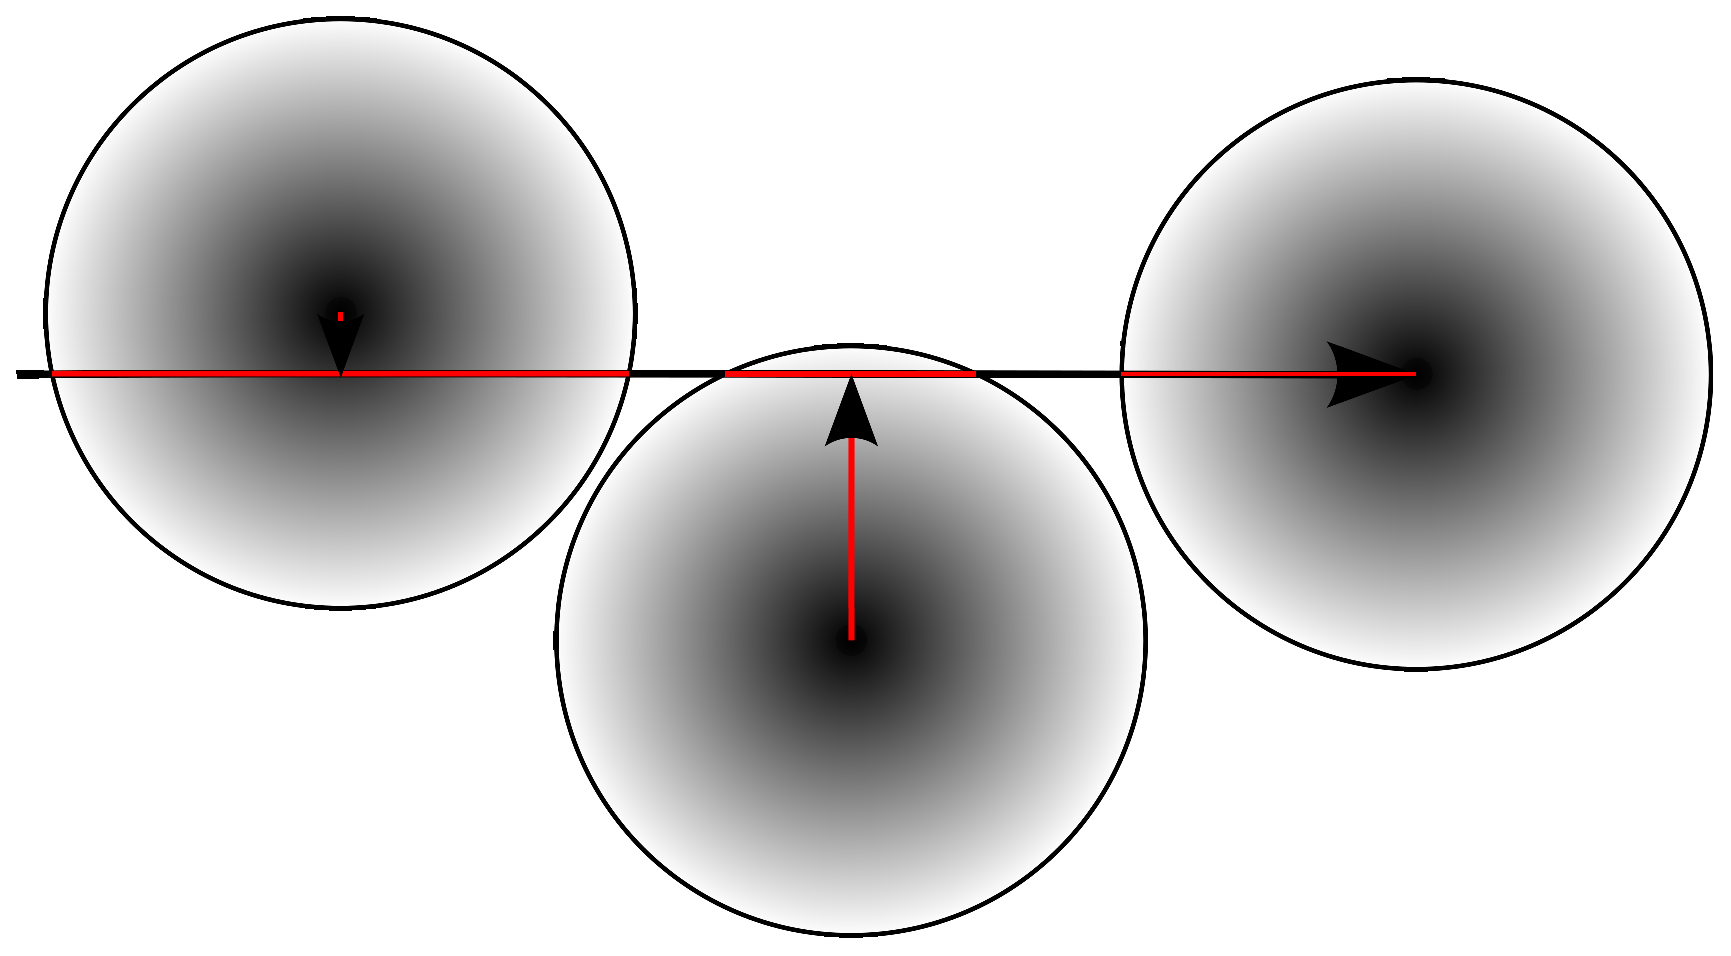
\includegraphics[width=\textwidth]{graphics/raytrace.eps}
\caption[Ray tracing schemes for receiving cells.]{Two ray tracing schemes. The first is the scheme of \citet{altayEt08} in which the photons are diminished by optical depth along each particle's smoothing length that they pass through. The second scheme is much simpler and yields very similar results. It relies on the fact that the ray actually represents a very large cone of photons, and that most particles in the cell will probably contribute to the absorption of photons at the receiving particle. It essentially simplifies to setting b = 0 for every particle in the receiving leaf.}
\label{fig:raytracing}
\end{figure}

Introducing the ray tracing machinery for the above purpose also creates the ability to ray trace within leaves during the refine mentioned in section \ref{sec:refinement}. In principle, this means the code can easily be forced into a full ray trace if this behavior is desired.

\subsection{High Optical Depth Particles}
\label{sec:hightau}

High tau particles are problematic. This is how we deal with them...

\section{Periodicity}
\label{sec:periodicity}

Move to future work?

\section{Cosmological Background Radiation}
\label{sec:cosmobackground}

In order to do cosmological simulations properly, we must account for the radiation coming from the rest of the universe outside of the simulation volume. Most current codes apply a constant UV field to the entire box, essentially the lowest order approximation possible.
\begin{itemize}
\item Few codes have moved past this for cosmology, though some have.
\item OTVET \citep{petkovaSpringel09} uses their radiation scheme with periodic boundaries.
\item Other more detailed scheme apply a constant radiation field at the boundaries coming into the volume (add citations).
\item While our scheme is perfectly capable of doing a periodic option, we have opted to set up a number of ``background sources.'' The sources are distributed on the surface of a sphere at the very edge of the simulation (or larger if required) and the number of sources can be varied to match the required angular resolution of the background.
\item Finding the flux at the center of a sphere of sources is a problem akin to Newton's Shell Theorem. However, because the flux doesn't cancel like force, the solution does not work out the same. See equation \ref{eq:shellflux}.
\item Since the solution is logarithmic in r, the we can assume the flux is roughly constant at similar radii. Since most cosmological zoom simulations only consider gas at a fairly small radius, this is acceptable.
\end{itemize}

\begin{equation}
\label{eq:shellflux}
F = K\left[ \log{R+r} - ln(R-r) \right]
\end{equation}

\begin{figure}
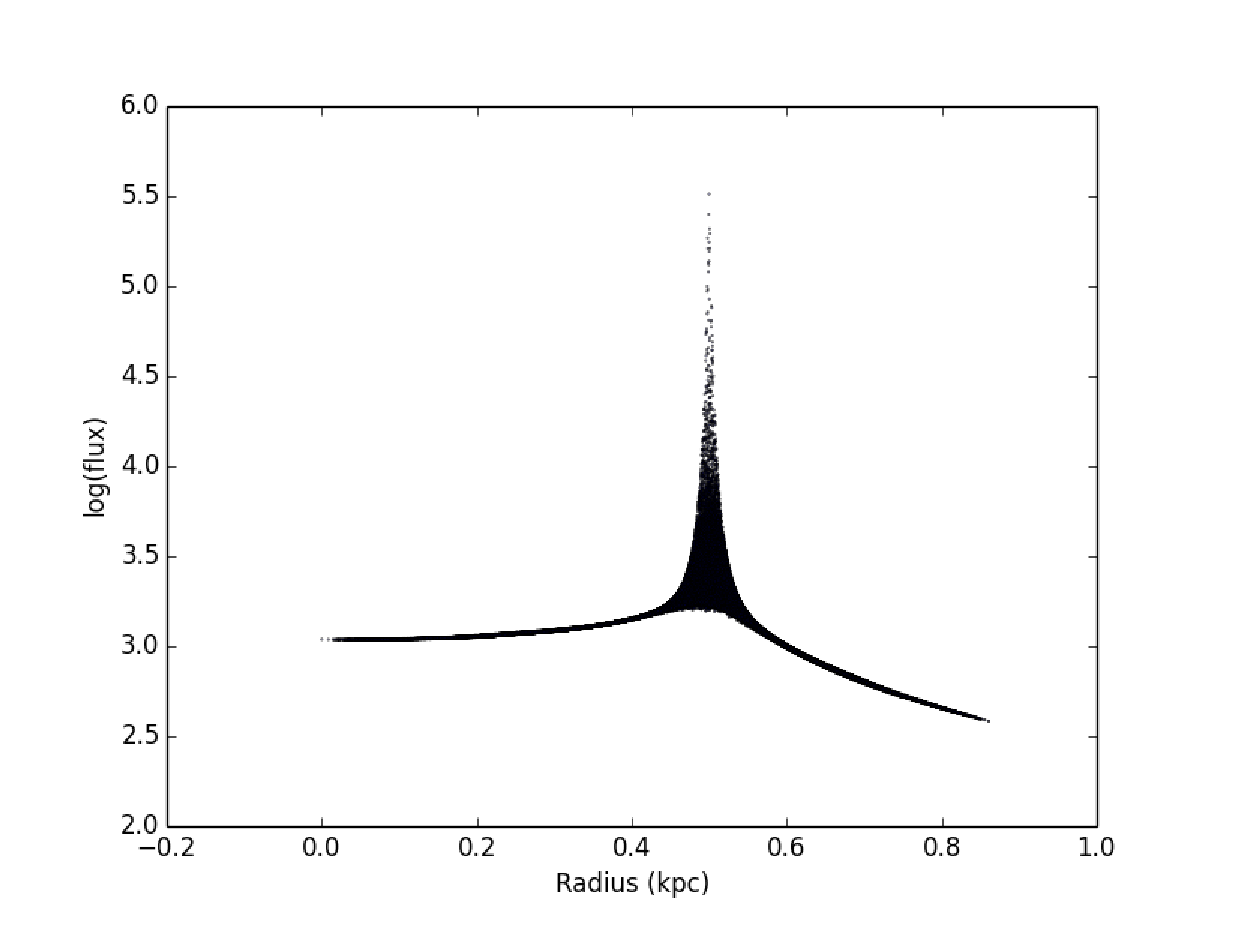
\includegraphics[width=\textwidth]{graphics/backgroundflux.eps}
\caption[Flux due to the cosmological background.]{The distribution of flux particles receive due to cosmological background particles when distributed in a sphere at the edge of the box. Note that value of the flux at the center can be easily scaled by simply scaling the luminosity of all sources on the sphere.}
\label{fig:backgroundflux}
\end{figure}

\section{Cosmological Effects}
\label{sec:cosmoeffects}
Move this section to ``future plans'' section?

\subsection{Cosmological Redshift of Radiation}
\label{sec:redshiftingradiation}


\subsection{Accounting for a Finite Speed of Light}
\label{sec:finitespeedoflight}

Move this section to ```future plans'' section?

\section{Summary of Algorithm}
\label{sec:algorithmsummary}

We have presented a flexible and computationally inexpensive algorithm for calculating the radiation field within a simulation. The algorithm affords many benefits (note: need to introduce many of stated benefits below in previous sections):

\begin{itemize}
\item It is flexible enough to allow a wide range of accuracy depending on the application. Speed starts at  $N\log{N}\log{N}$ and approaches that of ray tracing (check this...) when the algorithm is tuned to that level of refinement.
\item Because radiation is transferred instantaneously, the speed of light does not become a limiting time step. If ionization dynamics are important, then the propagation of the ionization front becomes the limiting time step. If only end behavior is required, then the there is very little the algorithm does to limit the time step.
\item There is no scan dependence. Because flux is accumulated at each receiving bucket without explicitly depositing the photons into the intervening material, ionization/heating/cooling is performed completely separate to radiation. This means that the solution will not change based on the order in which the sources are visited.
\item The algorithm is independent of wavelength or even number of wavelengths. The algorithm need only perform the tree walk and tree climb a single time in order to obtain the line segments in each cell. Performing different wavebands simply equates to recording multiple average opacities. This enables multi-band radiative transfer at little additional cost.
\end{itemize}

However, it is important to keep in mind the limitations and assumptions of this algorithm.
\begin{itemize}
\item Photons are not explicitly conserved. In order to save computational time, we can not keep track of the photons deposited in intervening material during an exchange. We obtain an optical depth and simply assume that the photons lost in the process have been deposited in the intervening material. When the intervening material is the receiving bucket at a later point in the algorithm, it should receive roughly the correct number of photons due to a matching initial segment (wording...).
\item Light is transferred instantaneously, meaning that photon fronts could travel faster than allowed, and that sinks could receive photons from a source too far away to have sent photons there yet.
\item Very large opacities in single particles can be problematic for both cooling (calculating the emitted flux from a particle is complex if the particle itself is optically thick) and ionization propagation. Particle self-absorption can impart the same ``stall'' in a single particle that was mentioned in section \ref{sec:resolvingleaves} for leaves.
\item Extra computation time can be required in the heating and cooling code due to intense local radiation fields. However, if the goal is to obtain a radiation field, this is already a built in cost to any algorithm. We simply mention it to suggest that increased computation time is due not only to the radiation algorithm, but the increased computation time for the cooling integrations (remove this point?). 
\end{itemize}

